\documentclass[twocolumn,aps]{revtex4}
\usepackage{amsmath}
\usepackage[utf8]{inputenc}
\usepackage[T1]{fontenc}
\usepackage{lmodern}
\usepackage[ngerman]{babel}
\usepackage{graphicx}
\graphicspath{{./img/}}
\begin{document}
\title{Kräfte im hängenden Seil}
\author{Gert-Ludwig Ingold}
\affiliation{Institut für Physik, Universität Augsburg, 86135 Augsburg}
\begin{abstract}
 In diesen Notizen soll die maximale Kraft hergeleitet werden, die in
 einem undehnbaren hängenden Seil auftritt. Dazu wird zunächst
 mit Hilfe der Betrachtung der auf ein kurzes Seilstück
 wirkenden Kräfte die Seilkurve hergeleitet. Anschließend lässt sich die
 maximale Seilkraft bestimmen.
\end{abstract}
\maketitle

\section{Kräftegleichgewicht an einem Seilstück}
Zunächst wird der Seilkurve eines undehnbaren, im Gravitationsfeld
hängenden Seils, berechnet. Es handelt sich dabei um ein
Variationsproblem mit Nebenbedingungen, in dem die potentielle Energie
des Seils bei vorgegebener Seillänge $L$ minimiert werden soll. Dies
kann mit Hilfe von Lagrange-Multiplikatoren und der zugehörigen
Euler-Lagrange-Gleichung erfolgen.  Da wir uns aber in erster Linie
für die Seilkräfte interessieren, ist es angebracht, die Seilkurve
stattdessen durch eine Kräftebetrachtung herzuleiten.

Wir beginnen mit der Betrachtung der in Abb.~\ref{fig:kraefte}
dargestellten Kräfte auf ein kurzes Seilstück der Länge $\mathrm{d}s$,
das sich am Ort $x_0$ befindet. Auf dieses Seilstück mit der
längenbezogenen Dichte $\mu$ wirkt die Gewichtskraft, die in die
negative $y$-Richtung zeigt und den Betrag
\begin{equation}
 G = \mu g\mathrm{d}s
\end{equation}
besitzt. Dabei ist $g$ die Erdbeschleunigung. Zudem üben die links und
rechts benachbarten Seilstücke die Kräfte $\vec F^{(-)}$ bzw.\ $\vec
F^{(+)}$ aus. Da das Seil keine Querkräfte zulassen soll, wirken diese
Kräfte in Richtung der jeweiligen Seilstücke. Im Gleichgewicht gilt
somit
\begin{equation}
 \vec F^{(+)}+\vec F^{(-)}+\vec G = 0\,.
 \label{eq:kraftgleichgewicht}
\end{equation}

\begin{figure}
 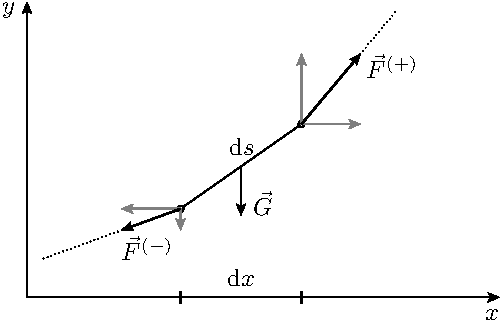
\includegraphics[width=0.8\columnwidth]{kraefte}
 \caption{Auf ein kurzes Seilstück der Länge $\mathrm{d}s$ wirken
	  die Gewichtskraft $\vec G$ sowie die Seilkräfte $\vec F^{(-)}$
	  und $\vec F^{(+)}$ von links bzw.\ von rechts. Die grau
	  dargestellten Vektoren zerlegen die Seilkräfte in die
	  horizontalen und vertikalen Komponenten.}
 \label{fig:kraefte}
\end{figure}

Diese Gleichgewichtsbedingung wird nun in ihre horizontalen und
vertikalen Komponenten zerlegt, wobei die Zerlegung der Seilkräfte in
Abb.~\ref{fig:kraefte} durch die grauen Vektoren dargestellt ist. Da
die Gewichtskraft keine horizontale Komponente besitzt, folgt
\begin{equation}
 F^{(+)}_x = -F^{(-)}_x = \mu g a\,.
 \label{eq:kraftgleichgewicht_x}
\end{equation}
Diese Kraftkomponente ist entlang des gesamten Seils konstant und wird
von der Aufhängung aufgebracht. Es ist günstig, die horizontale
Kraftkomponente in der angegebenen Form zu schreiben, wobei $a$ eine
Konstante mit der Dimension einer Länge ist, deren Bedeutung später
noch klar werden wird.

Beschreibt man die Seilkurve durch eine noch zu bestimmende Funktion
$y(x)$, so folgt aus der Tatsache, dass die Seilkräfte nur entlang des
Seils wirken können, dass das Verhältnis der Seilkraftkomponenten
gemäß
\begin{equation}
 \frac{F_y}{F_x} = \frac{\mathrm{d}y}{\mathrm{d}x} = y'(x)\,,
\end{equation}
durch die Ableitung der Seilkurve gegeben ist. Zur Vereinfachung der
Notation soll ein Strich die Ableitung nach der Koordinate $x$
bedeuten. Aus (\ref{eq:kraftgleichgewicht}) erhält man somit zusammen
mit (\ref{eq:kraftgleichgewicht_x}) für die vertikalen
Kraftkomponenten
\begin{equation}
 \mu ga\left[y'(x_0+\mathrm{d}x/2)-y'(x_0-\mathrm{d}x/2)\right]-\mu
 g\mathrm{d}s = 0\,.
\end{equation}
Hier sind wir von dem bisher verwendeten speziellen Ort $x_0$ des
Seilstücks zu einem beliebigen Ort $x$ übergegangen.

Dividiert man durch $\mathrm{d}x$, so wird aus der Differenz der
Ableitungen von $y(x)$ eine zweite Ableitung
\begin{equation}
 ay''(x)-\frac{\mathrm{d}s}{\mathrm{d}x} = 0\,.
 \label{eq:zweite_ableitung}
\end{equation}
Den Zusammenhang zwischen den Differentialen erhält man mit Hilfe des
Satzes von Pythagoras, der auf unser Problem angewandt als
\begin{equation}
 \mathrm{d}s^2 = \mathrm{d}x^2+\mathrm{d}y^2
\end{equation}
geschrieben werden kann. Daraus folgt
\begin{equation}
 \mathrm{d}s = \sqrt{1+y'(x)^2}\mathrm{d}x\,,
 \label{eq:ds}
\end{equation}
so dass wir mit (\ref{eq:zweite_ableitung}) die Differentialgleichung
der Seilkurve
\begin{equation}
 ay''(x)-\sqrt{1+y'(x)^2} = 0
 \label{eq:seilkurve_dgl}
\end{equation}
erhalten.

\section{Lösung der Seilkurvengleichung}
Die Differentialgleichung (\ref{eq:seilkurve_dgl}) lässt sich mit Hilfe der
Trennung der Variablen lösen, wenn man die neue Variable $u(x) = y'(x)$
einführt. Durch Trennung der Variablen erhält man
\begin{equation}
 \frac{\mathrm{d}u}{\sqrt{1+u^2}} = \frac{\mathrm{d}x}{a}\,.
\end{equation}
Die Integration dieser Gleichung liefert mit
\begin{equation}
 \int\mathrm{d}u\frac{1}{\sqrt{1+u^2}} = \mathrm{arsinh}(u)\,,
\end{equation}
wobei arsinh den inversen hyperbolischen Sinus bedeutet. Auflösen nach der
Variable $u$ liefert
\begin{equation}
 u = \sinh\left(\frac{x}{a}\right)\,.
 \label{eq:seilkurve_u}
\end{equation}
Eine potentiell auftretende Integrationskonstante haben wir hier zu Null
gesetzt und damit festgelegt, dass sich der tiefste Punkt des Seils am
Ort $x=0$ befindet.

Eine weitere Integration nach $x$ liefert schließlich die Seilkurve
\begin{equation}
 y= a\cosh\left(\frac{x}{a}\right)\,.
 \label{eq:seilkurve}
\end{equation}
Hier haben wir wiederum die Integrationskonstante zu Null gesetzt und
damit den tiefsten Punkt des Seils nach $y=0$ gelegt.

\section{Krümmungsradius}
Der Krümmungsradius $r$ einer durch die Funktion $y(x)$ beschriebenden
Kurve ist durch
\begin{equation}
 r(x) = \left\vert\frac{(1+y'(x)^2)^{3/2}}{y''(x)}\right\vert
\end{equation}
gegeben. Unter Verwendung der Ableitung der Seilkurve
(\ref{eq:seilkurve_u}) und mit der Beziehung
\begin{equation}
 \cosh(x)^2+\sinh(x)^2 = 1
\end{equation}
ergibt sich
\begin{equation}
 r(x) = a\cosh^2\left(\frac{x}{a}\right)\,.
\end{equation}
Der Parameter $a$ entspricht somit dem Krümmungsradius der Seilkurve
bei $x=0$, also am tiefsten Punkt. Dort ist der Krümmungsradius
minimal, die Krümmung also maximal.

Auch wenn sich der Krümmungsradius am tiefsten Punkt gut zur
Parametrisierung der Seilkurve eignet, wird er selten in
Problemstellungen vorgegeben sein. Wir wollen ihn daher durch
geeignete Parameter ausdrücken und betrachten dazu speziell ein
Seil, dass zwischen den Orten $x=\pm w/2$ auf der gleichen Höhe
eingespannt ist. Der Seildurchgang $h$ ergibt sich in diesem Fall mit
Hilfe der Seilkurve (\ref{eq:seilkurve}) zu
\begin{equation}
 h = y(w/2)-y(0) = a\left[\cosh\left(\frac{w}{2a}\right)-1\right]\,.
 \label{eq:durchhang}
\end{equation}

Ferner benötigen wir die Länge des Seils, die gleich $L$ sein soll.
Wir kennen nach (\ref{eq:ds}) den Zusammenhang zwischen der Länge
eines kleinen Seilstücks und dem Differential $\mathrm{d}x$, so dass
wir durch Auf\/integration die Forderung
\begin{equation}
 L \overset{!}{=} \int_{-w/2}^{w/2}\mathrm{d}x\sqrt{1+y'(x)^2}
\end{equation}
erhalten. Durch Einsetzen der Ableitung der Seilkurve
(\ref{eq:seilkurve_u}) und Ausführung der Integration finden wir
\begin{equation}
 L = 2a\sinh\left(\frac{w}{2a}\right)
\end{equation}
oder
\begin{equation}
 \cosh\left(\frac{w}{2a}\right) = \sqrt{1+\left(\frac{L}{2a}\right)^2}\,.
\end{equation}
Mit (\ref{eq:durchhang}) ergibt sich der Seildurchhang zu
\begin{equation}
 h = \sqrt{a^2+\frac{L^2}{4}}-a\,.
\end{equation}
Auf\/lösen nach $a$ erlaubt es, den Krümmungsradius am tiefsten
Seilpunkt durch die Seillänge $L$ und den Seildurchhang $h$ gemäß
\begin{equation}
 a = \frac{h}{2}\left[\left(\frac{L}{2h}\right)^2-1\right]
\end{equation}
auszudrücken.

\end{document}
